\documentclass{bmvc2k}

\bmvcreviewcopy{}

\usepackage{amsmath,amssymb}
\usepackage{booktabs}
\usepackage{multirow}
\usepackage{graphicx}
\usepackage{url}

\title{Architecture Shapes Explanation:\\
A Cross-Domain Benchmark of Post-Hoc XAI Disagreement}

\addauthor{Anonymous BMVC Submission}{}{1}
\addinstitution{Anonymous Institution}
\runninghead{Anonymous}{Architecture Shapes Explanation}

\def\eg{\emph{e.g}\bmvaOneDot}
\def\Eg{\emph{E.g}\bmvaOneDot}
\def\etal{\emph{et al}\bmvaOneDot}
\newcommand{\ours}{\textsc{SpineXNet-Bench}}
\newcommand{\rsna}{RSNA-Lumbar}
\newcommand{\cub}{CUB-200}

\begin{document}
\maketitle

\begin{abstract}
Post-hoc visual explanation methods are widely used to justify image classifiers, yet different methods can highlight contradictory regions for the same prediction. This disagreement is especially risky in clinical vision, where saliency maps may create unwarranted confidence in automated decisions. We study whether such disagreement is merely method-specific noise or whether it is systematically shaped by model architecture. We introduce \ours, a two-domain benchmark spanning RSNA lumbar spine magnetic resonance imaging and CUB-200 fine-grained bird classification, with eight architectures, seven explanation methods, five-fold validation, expert-coordinate clinical alignment, model-randomization checks, and consensus explanation variants. Across both domains, explanation agreement follows a stable three-tier pattern: classic convolutional networks agree most strongly, modern convolutional networks form a domain-sensitive middle tier, and patch-based Transformers agree least. On RSNA, DenseNet-121 and ResNet-50 reach mean pairwise Spearman agreement of $0.434$ and $0.412$, while ViT-Small and DeiT-Small remain near $0.205$ and $0.203$ despite competitive classification AUCs. The pattern reproduces on CUB-200, where DenseNet-121 reaches $0.518$ and DeiT-Small remains lowest at $0.220$; the cross-domain architecture-rank correlation across the six shared architectures is $\rho_s=0.943$ ($p=0.0048$). Consensus helps: across all six CUB-200 architectures, faithfulness-weighted averaging improves insertion AUC over uniform averaging and oracle top-$3$ curation improves further; the same ordering holds in the repaired RSNA subset where all three variants are available. Finally, expert-coordinate overlap remains below $0.28$ IoU for post-hoc maps, while a controlled concept bottleneck model corrects $59.2\%$ of previously wrong RSNA predictions through concept intervention. These results argue that explanation reliability is not solely a property of the XAI method; it is constrained by the inductive bias of the underlying architecture.
\end{abstract}

\section{Introduction}

Deep image classifiers are increasingly evaluated not only by whether they predict correctly, but by whether their decisions can be inspected. In radiology, this pressure is direct: a model that grades lumbar spine degeneration must give clinicians some reason to trust, audit, or reject its prediction. In general computer vision, the same issue appears as a reproducibility and model-selection problem. If an explanation method says that a classifier used a bird's head while another method says it used the background, the system has not become transparent; it has produced a second layer of uncertainty.

The disagreement problem in explainable machine learning formalizes this concern: different post-hoc explanation methods can assign incompatible importance to the same input features for the same model prediction~\cite{krishna2022disagreement}. Prior work has shown that disagreement occurs and that explanation metrics themselves can be unstable~\cite{hedstrom2024latec,adebayo2018sanity}. Less is known about whether disagreement is organized by the classifier architecture. This distinction matters. If disagreement is mostly random variation across explanation methods, one might handle it by reporting several maps. If it is architecture-conditioned, then explanation reliability becomes part of architecture selection itself.

We test this hypothesis across two visually different domains. The first is the RSNA 2024 lumbar spine degenerative classification challenge, a safety-critical magnetic resonance imaging (MRI) task with five conditions, five disc levels, three severity grades, and expert coordinate annotations~\cite{rsna2024lumbar}. The second is CUB-200-2011, a fine-grained natural image benchmark with 200 bird categories and 11,788 images~\cite{wah2011cub}. This pairing is intentional: RSNA supplies the clinical trust setting, while CUB-200 tests whether the same architecture-disagreement structure survives outside medical imaging.

Figure~\ref{fig:gallery} illustrates the core phenomenon. The input and prediction are fixed, but the highlighted evidence changes sharply across explanation methods and architectures. Quantitatively, we evaluate Grad-CAM, Grad-CAM++, Integrated Gradients, GradientSHAP, Occlusion, Guided Backpropagation, and Attention Rollout where applicable. We benchmark ConvNeXt-Tiny, ResNet-50, DenseNet-121, EfficientNet-B4, ViT-Small, DeiT-Small, and two concept bottleneck variants on RSNA; the six black-box backbones are repeated on CUB-200.

\begin{figure}[t]
  \centering
  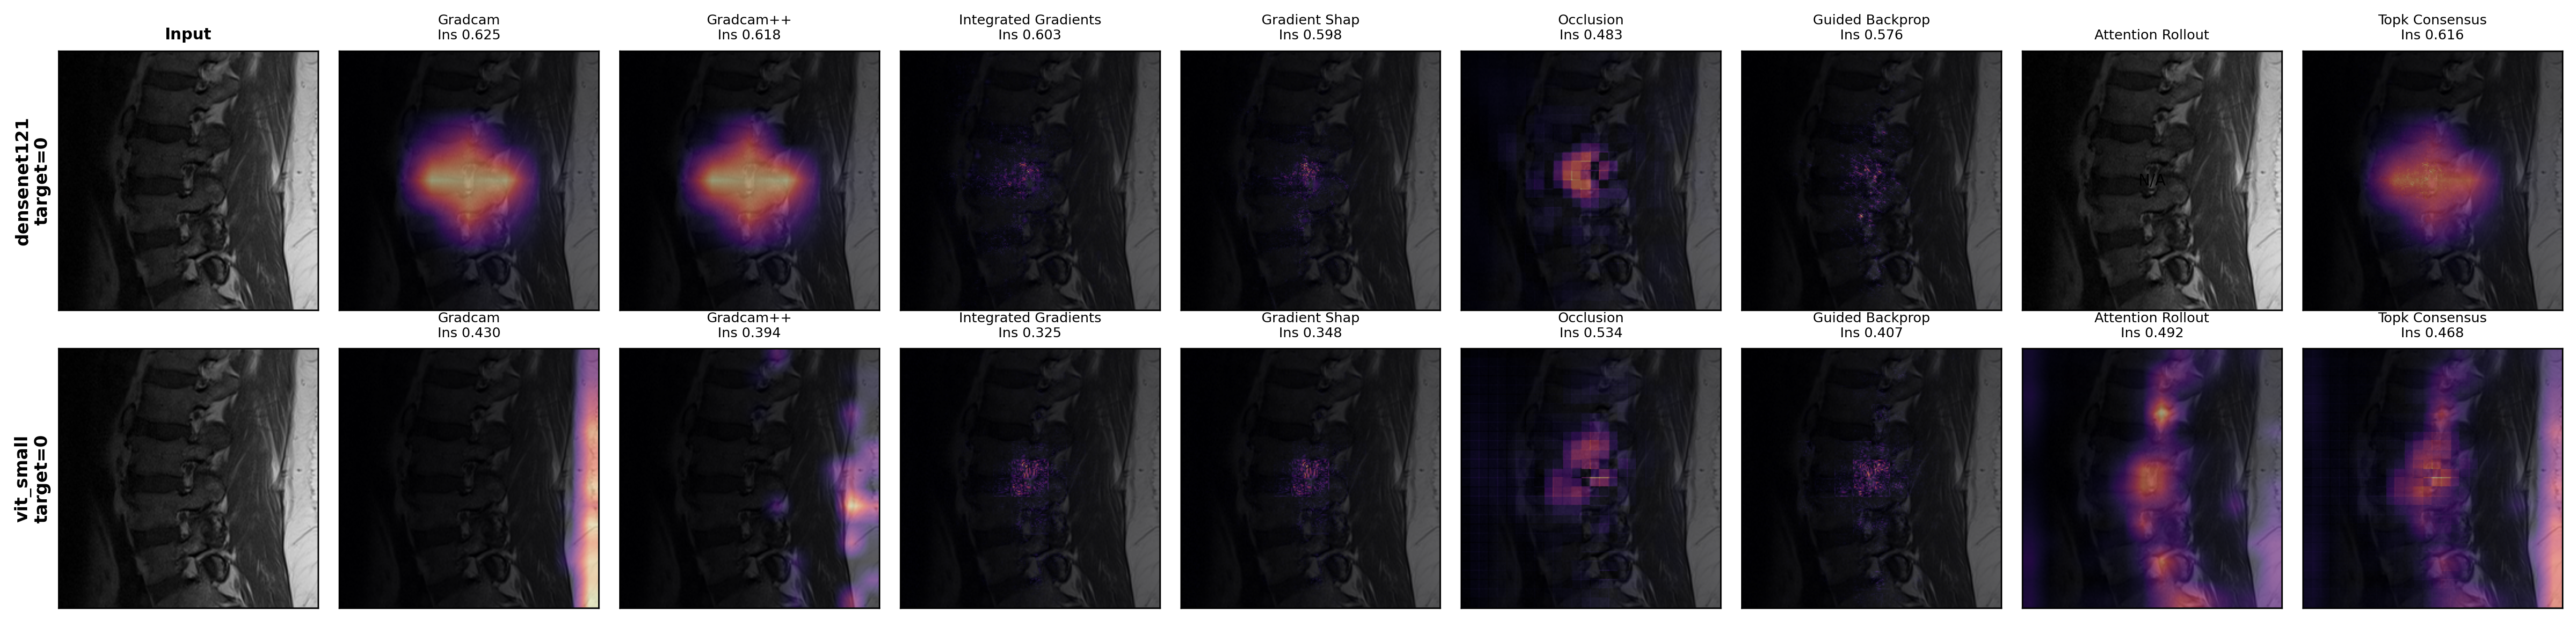
\includegraphics[width=\linewidth]{figures/figure1_disagreement_gallery.png}
  \caption{Qualitative explanation disagreement on RSNA lumbar spine MRI. For a fixed fold-0 sample and target prediction, post-hoc explanation methods produce visibly different saliency patterns across DenseNet-121 and ViT-Small. Attention Rollout is Transformer-native and is therefore not applicable to CNN rows. The gallery motivates the benchmark question studied in this paper: whether such disagreement is method noise alone or whether it is systematically shaped by model architecture.}
  \label{fig:gallery}
\end{figure}

Our findings support a three-tier architecture view rather than a strict universal ranking. Classic convolutional networks, represented by DenseNet-121 and ResNet-50, consistently show the highest inter-method agreement. Modern convolutional networks, represented by ConvNeXt-Tiny and EfficientNet-B4, move between the high- and low-agreement groups depending on domain. Patch-based Transformers, represented by ViT-Small and DeiT-Small, consistently show the weakest agreement. DeiT-Small is particularly important because it is trained by distillation from a convolutional teacher~\cite{touvron2021training}; its low agreement indicates that the pattern is not a ViT-Small artifact.

We make three contributions.
\begin{enumerate}
  \item We introduce a cross-domain benchmark for post-hoc XAI disagreement across RSNA lumbar MRI and CUB-200, covering eight architectures, seven explanation methods, expert-coordinate clinical alignment, and five-fold validation.
  \item We show that explanation disagreement is architecture-class dependent and statistically stable: classic CNNs form a high-agreement tier, modern CNNs are domain-sensitive, and ViT-Small with DeiT-Small forms a low-agreement Transformer tier. DenseNet-121 exceeds ViT-Small by $\Delta\rho=0.229$ on RSNA ($p=4.99{\times}10^{-4}$) and by $\Delta\rho=0.235$ on CUB-200 ($p=1.55{\times}10^{-5}$); RSNA and CUB architecture ranks correlate across the six shared architectures ($\rho_s=0.943$, $p=0.0048$).
  \item We evaluate practical responses to disagreement. Faithfulness-weighted consensus is compared with uniform averaging, oracle top-$3$ consensus estimates the value of method curation, and a controlled concept bottleneck model enables intervention that fixes $59.2\%$ of previously wrong RSNA predictions.
\end{enumerate}

\section{Related Work}

\paragraph{Post-hoc visual explanations.}
Saliency methods estimate which input regions support a prediction. Gradient-based saliency traces derivatives with respect to pixels~\cite{simonyan2014deep}; Integrated Gradients accumulates gradients from a baseline to the input and satisfies attribution axioms~\cite{sundararajan2017axiomatic}; and GradientSHAP estimates SHAP-style attributions through noisy gradient sampling. Perturbation approaches such as occlusion remove or reveal image regions and measure the output change~\cite{zeiler2014visualizing}. Class activation mapping methods, including Grad-CAM and Grad-CAM++, localize class evidence through convolutional feature maps~\cite{selvaraju2017gradcam,chattopadhay2018gradcampp}. For Transformers, Attention Rollout aggregates attention flow through layers~\cite{abnar2020quantifying}. These methods are often treated as interchangeable explanations of a fixed prediction, but their computational assumptions differ substantially.

\paragraph{Explanation disagreement and benchmark reliability.}
Krishna \etal formalized explanation disagreement and showed that practitioners lack principled ways to resolve conflicting explanations~\cite{krishna2022disagreement}. Adebayo \etal demonstrated that some saliency maps can fail model-parameter sanity checks~\cite{adebayo2018sanity}. Recent large-scale XAI benchmarks such as LATEC evaluate explanation methods and metrics across broad method-metric grids~\cite{hedstrom2024latec}. Our focus is orthogonal: we ask whether inter-method explanation disagreement is shaped by architecture class and whether the resulting hierarchy reproduces across clinical and natural image domains. Thus, while LATEC studies metric reliability at scale, our work studies architecture-conditioned disagreement, cross-domain stability, and expert-coordinate alignment.

\paragraph{Architecture and inductive bias.}
Modern vision models differ in spatial inductive bias. ResNet and DenseNet rely on convolutional locality and hierarchical feature reuse~\cite{he2016resnet,huang2017densenet}. EfficientNet uses compound scaling of depth, width, and resolution~\cite{tan2019efficientnet}, while ConvNeXt modernizes convolutional design choices in response to Transformer-era architectures~\cite{liu2022convnet}. ViT and DeiT tokenize images into patches and use self-attention rather than convolutional spatial aggregation~\cite{dosovitskiy2021image,touvron2021training}. These architectural differences motivate our central question: do explanation methods disagree differently when the classifier computation itself changes?

Concurrent work on hypothesis-class effects reaches a related conclusion from the opposite experimental direction~\cite{thackshanaramana2026hypothesis}. That work fixes the attribution setting and varies prediction-equivalent model classes, showing that models from the same hypothesis class produce more consistent feature attributions than cross-class model pairs. Our study fixes each trained vision model and varies the explanation method, then tests whether the resulting inter-method disagreement hierarchy reproduces across clinical MRI and fine-grained natural images. The overlap is therefore the broad principle that model class is not explanation-neutral; the difference is that we study within-model method disagreement, cross-domain visual evidence, and clinical expert-coordinate alignment.

\paragraph{Concept bottlenecks.}
Concept bottleneck models (CBMs) predict human-interpretable concepts before making a final prediction and support intervention by editing concept values~\cite{koh2020concept}. In health care, however, post-hoc explanations can create a false sense of interpretability if they do not correspond to clinically meaningful evidence~\cite{ghassemi2021false}. We therefore treat the CBM in this paper as a controlled ante-hoc alternative rather than simply another saliency method. Because our concepts are deterministic and metadata-derived, this choice isolates architecture and explanation-method effects without adding a noisy concept-discovery problem.

\section{Benchmark Design}

\subsection{Datasets}

\textbf{RSNA lumbar spine MRI.} We use the RSNA 2024 Lumbar Spine Degenerative Classification task~\cite{rsna2024lumbar}. The benchmark contains approximately 2,697 patients and condition-level crops from lumbar MRI studies. Each crop is associated with one of five degenerative conditions, one of five disc levels, and one of three severity grades. The final manifest contains 48,657 condition-level samples, resized to $224{\times}224$ and converted to three-channel tensors for ImageNet-pretrained backbones. Splits are stratified five-fold patient-level splits. Expert $(x,y)$ coordinates are used to construct circular region-of-interest masks for clinical alignment.

\textbf{CUB-200.} CUB-200-2011 is a fine-grained natural image benchmark with 11,788 images across 200 bird species~\cite{wah2011cub}. We use stratified five-fold validation rather than the official train/test split so that agreement statistics can be paired across folds. Images are resized and center-cropped to $224{\times}224$ at validation time. The CUB task tests whether the RSNA architecture-disagreement hierarchy is a clinical-domain artifact or a more general computer-vision phenomenon.

The implementation, experiment scripts, and aggregate outputs are available at \url{https://github.com/tanvishdesai/spinexhet}.

\subsection{Architectures}

RSNA includes eight models: ConvNeXt-Tiny, ResNet-50, DenseNet-121, EfficientNet-B4, ViT-Small, DeiT-Small, a non-leaky CBM, and a leaky CBM ablation. CUB-200 includes the six black-box backbones; CBMs are excluded because the RSNA metadata concepts do not transfer to bird species recognition. DeiT-Small is the second Transformer and is crucial to the benchmark: it has a ViT-like patch-token architecture but a different training paradigm based on distillation~\cite{touvron2021training}.

All RSNA models use condition and level embeddings concatenated to visual features. Black-box classifiers use a pretrained \texttt{timm} backbone with global average pooling, a hidden dimension of 256, dropout $0.2$, and an optional CORAL-style ordinal head. The CBM predicts seven non-leaky metadata-derived concepts from ConvNeXt-Tiny features and condition/level embeddings, then predicts severity from concept probabilities and metadata. We interpret this as a controlled concept-intervention baseline, not as evidence that visual concept discovery has been solved.

\begin{figure*}[t]
  \centering
  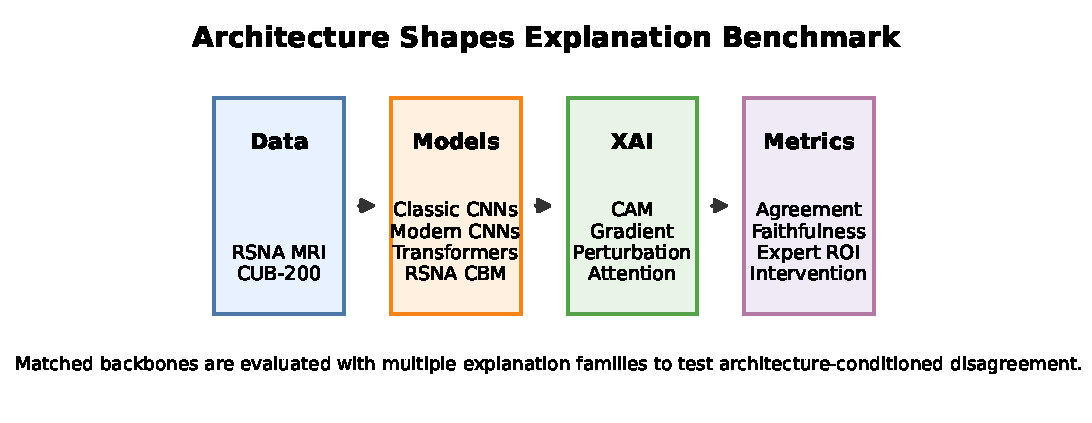
\includegraphics[width=\textwidth]{figures/architecture_shapes_explanation.pdf}
  \caption{Benchmark schematic. RSNA lumbar MRI crops and CUB-200 bird images feed matched architecture families, after which post-hoc explanation maps are evaluated for inter-method agreement, faithfulness and consensus behavior, clinical expert-coordinate alignment, and concept intervention when a CBM is available.}
  \label{fig:method}
\end{figure*}

\subsection{Training Details}

RSNA models are trained with AdamW, ImageNet normalization, batch size 16, gradient accumulation 2, automatic mixed precision, class-weighted cross entropy, and ordinal loss weight $0.2$. Baseline CNNs use learning rate $10^{-3}$ and backbone learning rate $10^{-4}$; DeiT-Small uses backbone learning rate $5{\times}10^{-5}$. Warmup lasts 5 epochs, early stopping patience is 10 epochs, and the random seed is 42. RSNA data augmentation includes horizontal flip, rotation up to $10^\circ$, small affine translation/scale, brightness/contrast jitter, and random erasing.

CUB models use AdamW with pretrained \texttt{timm} backbones, random resized crop, horizontal flip, mild color jitter, ImageNet normalization, label smoothing, and cosine scheduling. The default recipe trains for 15 epochs with learning rate $3{\times}10^{-4}$. ConvNeXt-Tiny and DeiT-Small use a gentler recipe: 30--35 epochs, backbone learning rate $5{\times}10^{-5}$, head learning rate $5{\times}10^{-4}$, warmup 3 epochs, drop-path $0.1$, and patience 8.

\subsection{Explanation Methods and Metrics}

For each trained model and fold, we compute Grad-CAM, Grad-CAM++, Integrated Gradients, GradientSHAP, Occlusion, Guided Backpropagation, and, for ViT/DeiT, Attention Rollout. Attribution maps are normalized to $[0,1]$ and resized to the input resolution. Inter-method agreement is measured as the mean pairwise Spearman correlation over flattened attribution maps and as top-20\% saliency IoU. Faithfulness is measured by deletion and insertion curves; higher insertion AUC indicates that revealing highly attributed pixels restores the target confidence quickly. Clinical alignment on RSNA is the IoU between the top saliency pixels and an expert-coordinate ROI.

\paragraph{Consensus.}
Given maps $A_i$ and insertion AUC weights $w_i$, faithfulness-weighted consensus is
\begin{equation}
  A_{\mathrm{FW}} = \frac{\sum_i w_i A_i}{\sum_i w_i}.
\end{equation}
Uniform consensus sets all weights equal. The oracle top-$k$ variant keeps the $k=3$ most faithful methods for the same sample before applying the same weighted average. Because this selector uses the sample's own insertion AUC, we treat it as an upper-bound ablation for the value of method curation, not as a claim that per-sample top-$k$ selection is already a low-cost deployment protocol. A deployable variant would select a fixed top-$k$ method set per architecture from validation-set mean faithfulness. All six CUB-200 architectures have faithfulness-weighted, uniform, and oracle top-$3$ consensus metrics; on RSNA, all three variants are available for EfficientNet-B4, DeiT-Small, and the repaired ViT-Small folds, while the remaining RSNA models retain faithfulness-weighted consensus.

\section{Results}

\subsection{Classification Competence}

Before interpreting explanations, each architecture must be a competent classifier. Table~\ref{tab:classification} reports five-fold classification performance. On RSNA, ConvNeXt-Tiny achieves the best weighted log loss (0.511) and AUC-OVR (0.920), while ViT-Small, DeiT-Small, DenseNet-121, and the non-leaky CBM all remain near AUC 0.916--0.920. On CUB-200, all six models exceed the 70\% XAI inclusion threshold; ConvNeXt-Tiny reaches $90.7\%$ accuracy and DeiT-Small reaches $87.3\%$.

\begin{table}[t]
\centering
\small
\begin{tabular}{lcccc}
\toprule
\multirow{2}{*}{Model} & \multicolumn{2}{c}{RSNA} & \multicolumn{2}{c}{CUB-200}\\
\cmidrule(lr){2-3}\cmidrule(lr){4-5}
 & WLL $\downarrow$ & AUC-OVR $\uparrow$ & Acc. $\uparrow$ & Top-5 $\uparrow$\\
\midrule
ConvNeXt-Tiny & \textbf{0.511} $\pm$ .012 & \textbf{0.920} $\pm$ .007 & \textbf{90.7} $\pm$ .6 & \textbf{97.6} $\pm$ .2\\
DenseNet-121 & 0.531 $\pm$ .015 & 0.916 $\pm$ .003 & 83.3 $\pm$ .6 & 95.6 $\pm$ .3\\
ResNet-50 & 0.572 $\pm$ .012 & 0.902 $\pm$ .005 & 84.4 $\pm$ .9 & 96.4 $\pm$ .4\\
EfficientNet-B4 & 0.650 $\pm$ .016 & 0.882 $\pm$ .011 & 84.5 $\pm$ .4 & 95.9 $\pm$ .2\\
ViT-Small & 0.525 $\pm$ .017 & 0.916 $\pm$ .006 & 74.8 $\pm$ 5.8 & 90.6 $\pm$ 2.9\\
DeiT-Small & 0.520 $\pm$ .011 & 0.916 $\pm$ .004 & 87.3 $\pm$ .2 & 96.4 $\pm$ .1\\
CBM non-leaky & 0.539 $\pm$ .010 & 0.920 $\pm$ .008 & -- & --\\
\bottomrule
\end{tabular}
\caption{Classification performance. RSNA uses weighted log loss (WLL) and one-vs-rest multiclass AUC; CUB-200 reports top-1 and top-5 accuracy. All non-CBM architectures are sufficiently trained for explanation analysis.}
\label{tab:classification}
\end{table}

\subsection{Architecture-Dependent Explanation Agreement}

Table~\ref{tab:agreement} is the main result. RSNA agreement separates into three tiers. DenseNet-121 and ResNet-50 are highest, with mean Spearman $\rho=0.434$ and $0.412$. ConvNeXt-Tiny and EfficientNet-B4 form a lower, domain-sensitive middle on RSNA, with $\rho=0.283$ and $0.223$. ViT-Small and DeiT-Small are lowest, with $\rho=0.205$ and $0.203$. The DeiT result is not explained by poor classification: DeiT's RSNA AUC is $0.916$, comparable to ViT and DenseNet.

The CUB-200 results reproduce the same family-level structure. DenseNet-121 remains highest ($\rho=0.518$), ResNet-50 remains high ($\rho=0.430$), and DeiT-Small remains lowest ($\rho=0.220$). ConvNeXt-Tiny moves upward on CUB ($\rho=0.441$), confirming that modern CNNs are domain-sensitive rather than strictly ranked. The rank correlation between RSNA and CUB across the six shared architectures is $\rho_s=0.943$ (two-tailed $p=0.0048$, $n=6$).

\begin{figure}[t]
  \centering
  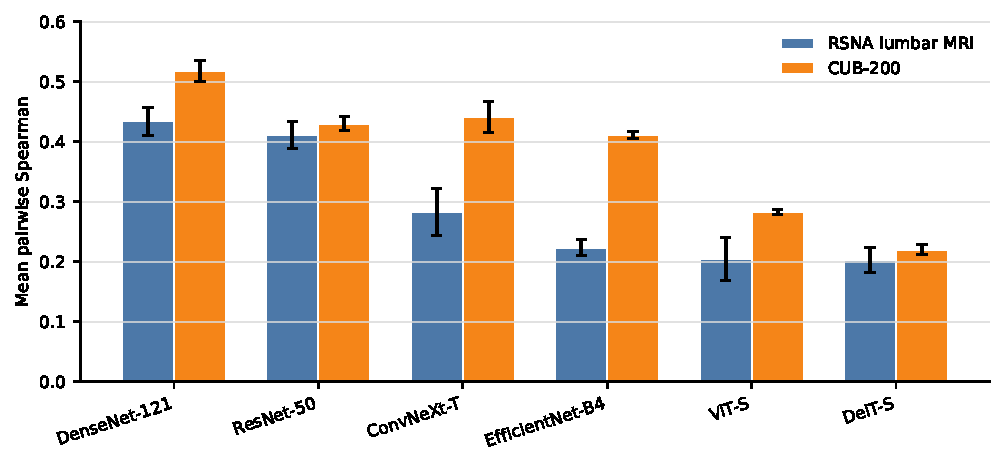
\includegraphics[width=.88\linewidth]{figures/agreement_hierarchy.pdf}
  \caption{Cross-domain explanation agreement hierarchy. Mean pairwise Spearman agreement between XAI methods shows a stable high-agreement classic CNN tier and a low-agreement Transformer tier across RSNA lumbar MRI and CUB-200. ConvNeXt and EfficientNet are domain-sensitive middle architectures rather than a fixed rank.}
  \label{fig:agreement}
\end{figure}

\begin{table}[t]
\centering
\small
\begin{tabular}{lcccc}
\toprule
Model & \multicolumn{2}{c}{RSNA} & \multicolumn{2}{c}{CUB-200}\\
\cmidrule(lr){2-3}\cmidrule(lr){4-5}
 & Spearman $\rho$ & Top-20 IoU & Spearman $\rho$ & Top-20 IoU\\
\midrule
DenseNet-121 & \textbf{0.434} $\pm$ .023 & \textbf{0.385} $\pm$ .014 & \textbf{0.518} $\pm$ .018 & \textbf{0.411} $\pm$ .009\\
ResNet-50 & 0.412 $\pm$ .023 & 0.329 $\pm$ .015 & 0.430 $\pm$ .012 & 0.382 $\pm$ .006\\
ConvNeXt-Tiny & 0.283 $\pm$ .039 & 0.326 $\pm$ .026 & 0.441 $\pm$ .026 & 0.383 $\pm$ .010\\
EfficientNet-B4 & 0.223 $\pm$ .013 & 0.231 $\pm$ .008 & 0.411 $\pm$ .006 & 0.348 $\pm$ .006\\
ViT-Small & 0.205 $\pm$ .036 & 0.239 $\pm$ .022 & 0.283 $\pm$ .004 & 0.297 $\pm$ .006\\
DeiT-Small & 0.203 $\pm$ .021 & 0.245 $\pm$ .013 & 0.220 $\pm$ .008 & 0.261 $\pm$ .005\\
\bottomrule
\end{tabular}
\caption{Mean inter-method explanation agreement over five folds for the six architectures shared across RSNA and CUB-200. Classic CNNs form the high-agreement tier, Transformers form the low-agreement tier, and modern CNNs shift with domain. RSNA-only CBM agreement is discussed with the intervention results.}
\label{tab:agreement}
\end{table}

\subsection{Statistical Tests}

The tier differences are robust by paired $t$-test across the key high-vs-low agreement comparisons (Table~\ref{tab:stats}). On RSNA, DenseNet-121 exceeds ViT-Small by $\Delta\rho=0.229$ (paired $t=10.31$, $p=4.99{\times}10^{-4}$) and DeiT-Small by $\Delta\rho=0.231$ ($p=1.09{\times}10^{-4}$). CUB-200 shows the same pattern: DenseNet-121 exceeds ViT-Small by $\Delta\rho=0.235$ ($p=1.55{\times}10^{-5}$) and DeiT-Small by $\Delta\rho=0.298$ ($p=4.33{\times}10^{-6}$). Wilcoxon signed-rank tests, which have limited resolution at $n=5$ folds, also assign all comparisons the minimum attainable two-sided value of $0.0625$.

\begin{table}[t]
\centering
\small
\begin{tabular}{lccc}
\toprule
Comparison & $\Delta\rho$ & Paired $t$ & $p$\\
\midrule
RSNA DenseNet-121 vs. ViT-Small & 0.229 & 10.31 & $4.99{\times}10^{-4}$\\
RSNA ResNet-50 vs. ViT-Small & 0.207 & 8.17 & $1.22{\times}10^{-3}$\\
RSNA DenseNet-121 vs. DeiT-Small & 0.231 & 15.22 & $1.09{\times}10^{-4}$\\
CUB DenseNet-121 vs. ViT-Small & 0.235 & 24.86 & $1.55{\times}10^{-5}$\\
CUB ResNet-50 vs. ViT-Small & 0.147 & 24.01 & $1.79{\times}10^{-5}$\\
CUB DenseNet-121 vs. DeiT-Small & 0.298 & 34.26 & $4.33{\times}10^{-6}$\\
\bottomrule
\end{tabular}
\caption{Fold-paired tests for high-agreement classic CNNs against low-agreement Transformers. All comparisons use five folds.}
\label{tab:stats}
\end{table}

\subsection{Consensus Explanations}

Consensus explanations are intended to reduce arbitrary dependence on a single XAI method, but they should not be interpreted as guaranteed improvements over the best individual method. In the full RSNA faithfulness-weighted analysis, the non-leaky CBM achieves the highest consensus insertion AUC ($0.826\pm0.034$), followed by ConvNeXt-Tiny ($0.810\pm0.020$) and DenseNet-121 ($0.808\pm0.024$). In the RSNA model-folds where all three variants are available after repair, oracle top-$3$ consensus improves over faithfulness-weighted consensus by $0.0169$ insertion AUC on average (paired $t$-test over 12 model-folds, $p=8.31{\times}10^{-5}$), while faithfulness weighting also improves over uniform averaging by $0.0031$ ($p=2.78{\times}10^{-4}$).

CUB-200 provides the cleaner all-architecture consensus check (Figure~\ref{fig:consensus}). Faithfulness-weighted consensus exceeds uniform averaging for all six backbones, with a mean gain of $0.0107$ insertion AUC across 30 model-folds ($p=1.72{\times}10^{-7}$). Oracle top-$3$ consensus further exceeds faithfulness-weighted consensus for every CUB architecture, with a mean gain of $0.0340$ ($p=1.11{\times}10^{-9}$). The largest top-$3$ gains appear for ResNet-50 ($0.699$ versus $0.642$) and ViT-Small ($0.541$ versus $0.488$), suggesting that method curation can matter even for otherwise stable CNNs and is especially useful when individual explanation methods disagree.

\begin{figure}[t]
  \centering
  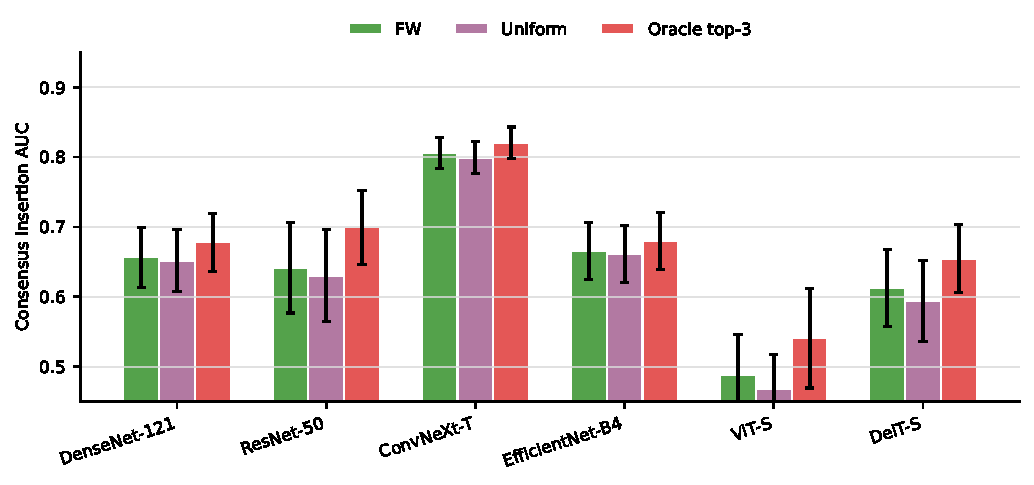
\includegraphics[width=.86\linewidth]{figures/consensus_ablation.pdf}
  \caption{CUB-200 consensus ablation across all six architectures. Faithfulness-weighted (FW) consensus is consistently above uniform averaging, and oracle top-$3$ consensus is higher still. Because top-$3$ uses sample-level insertion AUC for selection, it should be read as an upper-bound estimate for method curation rather than as a deployable inference protocol. Error bars indicate fold-level standard deviation.}
  \label{fig:consensus}
\end{figure}

This result changes the practical recommendation while preserving a clear distinction between deployable and oracle variants. Averaging all explanations is not necessarily optimal: low-faithfulness maps can dilute useful evidence. A practical system should select a fixed set of reliable methods from validation-set faithfulness, while the present oracle top-$k$ ablation estimates how much room such curation has to help.

\subsection{Clinical Alignment and Concept Intervention}

Expert-coordinate alignment on RSNA remains low for all post-hoc explanations. The best mean consensus expert IoU is DenseNet-121 at $0.275\pm0.002$, followed by ResNet-50 at $0.265\pm0.008$ and the non-leaky CBM at $0.264\pm0.017$. EfficientNet-B4 reaches $0.260\pm0.006$, DeiT-Small reaches $0.255\pm0.005$, and ViT-Small reaches $0.224\pm0.013$. The correct interpretation is not that post-hoc maps are clinically aligned, but that even the best average overlap with expert-localized pathology remains below 30\%.

If disagreement is intrinsic to post-hoc explanations for some architecture classes, ante-hoc interpretability becomes attractive not merely for transparency but for stability and intervention. The concept bottleneck model offers this different interaction mode. On 1,000 RSNA validation samples, the non-leaky CBM is initially correct on 848 samples. Of the 152 wrong predictions, editing one concept can correct 90, yielding a $59.2\%$ fix rate (Table~\ref{tab:cbm}). The most useful concept is adjacent pathology density, which alone fixes $51.3\%$ of the wrong cases. The leaky CBM achieves a higher intervention fix rate, but its dominant concept encodes pathology presence and is therefore treated only as an ablation.

\begin{table}[t]
\centering
\small
\begin{tabular}{lcc}
\toprule
Intervention statistic & Non-leaky CBM & Leaky CBM\\
\midrule
Wrong predictions before intervention & 152 & 162\\
Fixable by any single concept & 90 & 137\\
Fix rate & \textbf{59.2\%} & 84.6\%\\
Dominant concept & adjacent pathology density & pathology present\\
Dominant concept fix rate & 51.3\% & 74.1\%\\
\bottomrule
\end{tabular}
\caption{RSNA concept-intervention summary. The non-leaky CBM is the primary controlled ante-hoc baseline; the leaky CBM is reported only as an ablation because its strongest concept encodes pathology presence.}
\label{tab:cbm}
\end{table}

\subsection{Negative and Diagnostic Results}

Two negative results are important for interpreting the benchmark. First, feature-map coherence did not explain the full architecture hierarchy: the correlation between feature coherence and agreement is weak across all architectures, though it matches the CNN ordering more closely. This suggests that Transformer disagreement is not captured by smoothness of intermediate features alone. Second, EfficientNet-B4 remains a domain-sensitive middle-tier architecture rather than a failed run: an audit of the initially suspicious Integrated Gradients and GradientSHAP scores confirmed non-identical maps, non-zero input gradients, and baseline-sensitive but valid attribution behavior across the repaired folds.

\section{Discussion}

The central lesson is that explanation reliability is not solely a property of the XAI method; it is constrained by the inductive bias of the underlying architecture. The claim is empirical, not causal proof: we do not show that architecture alone determines saliency. However, across two domains, multiple folds, and independently trained backbones, architecture class is a strong organizing factor for inter-method agreement. This has practical consequences. A high-performing classifier can still be a poor candidate for post-hoc explanation if its saliency methods disagree severely.

The Transformer result is the most stable family-level finding. ViT-Small and DeiT-Small both occupy the low-agreement tier on RSNA and CUB-200. DeiT's low agreement is especially informative because distillation from a convolutional teacher does not make its explanations CNN-like. A plausible mechanism is that patch tokenization weakens the local spatial continuity that CAM and gradient methods exploit, while self-attention creates non-local evidence pathways that different attribution families interrogate differently. In contrast, DenseNet and ResNet preserve stronger convolutional locality and hierarchical feature reuse, which may stabilize where multiple attribution methods place evidence. Attention Rollout partly addresses this by using architecture-native attention flow, but the broader inter-method disagreement remains.

The domain-sensitive middle tier is also informative. EfficientNet shifts from low agreement on RSNA to a stronger middle position on CUB-200, and ConvNeXt similarly improves on CUB. This rank movement is consistent with the three-tier claim rather than a contradiction: compound scaling and modern convolutional design may behave differently on small, low-contrast MRI crops than on rich-texture natural images. The result cautions against strict architecture rankings while supporting architecture class as an organizing factor.

The consensus experiments show that resolving disagreement is not as simple as averaging every map. Faithfulness-weighted consensus is a principled baseline and consistently improves over uniform averaging in the completed CUB ablation, but oracle top-$3$ consensus performs better still. This suggests a general deployment rule: when explanations disagree, first identify methods that are faithful for the model and domain on validation data, then combine only that curated subset. The oracle result should be read as evidence that curation matters, not as a finished inference-time protocol.

The clinical results argue for caution. Post-hoc saliency maps overlap expert-coordinate regions less than 30\% of the time on average. This is not enough to support uncritical clinical deployment. The CBM result is useful because it shifts the user interaction from viewing a heatmap to editing a concept and observing the prediction change. Still, because our CBM concepts are deterministic metadata-derived concepts, the result should be read as evidence for controlled concept intervention rather than as a solved visual concept-learning system.

\section{Limitations}

The benchmark includes two Transformer architectures. ViT-Small and DeiT-Small are sufficient to rule out a single-model artifact, but Swin, CaiT, or hierarchical Transformers would strengthen family-level claims. The CUB consensus ablation is complete across all six backbones, while RSNA all-variant consensus remains available for EfficientNet-B4, DeiT-Small, and the repaired ViT-Small folds rather than every RSNA architecture. RSNA expert alignment uses coordinate-derived circular masks rather than dense radiologist segmentations. RSNA images cannot be redistributed freely under competition constraints, though the code, CUB pipeline, configurations, aggregate outputs, and model-release plan are available through \url{https://github.com/tanvishdesai/spinexhet}.

\section{Conclusion}

Post-hoc explanation disagreement is not merely a property of explanation methods in isolation. In our two-domain benchmark, architecture class strongly structures whether those methods agree. Classic convolutional networks produce comparatively stable explanations, modern convolutional networks are domain-sensitive, and patch-based Transformers show consistently low agreement even when classification performance is competitive. Consensus can reduce the burden of choosing a single map, but the oracle top-$3$ ablation shows that curation is more promising than unfiltered averaging. In safety-critical settings, low expert-coordinate overlap makes ante-hoc and intervention-based interpretability especially important. Architecture-aware explanation evaluation should therefore become part of model selection, not an afterthought applied after accuracy has already chosen the model.

\bibliography{egbib}

\end{document}
